\chapter{Fixes}

In phase 4, Team 13 performed White-box testing of our application. In their findings, they mentioned six issues to be fixed. They are as stated below.

\section{SCS Exception due to incorrect Java version} - This was a major flaw, as the Smart Card Simulator worked on Java version 1.8 and the version of Java on the Virtual Machine was 1.7. Though the SCS works without any issue after update of Java version, we considered to fix it anyway.
The fix involved making changes to the project properties for compatibility to version Java 1.7, before exporting the JAR. This was a minor change and required no modifications in code. Refer figure \ref{fig:fix_java_version}. \\ \\ \\

\begin{figure}[ht]
	\centering
	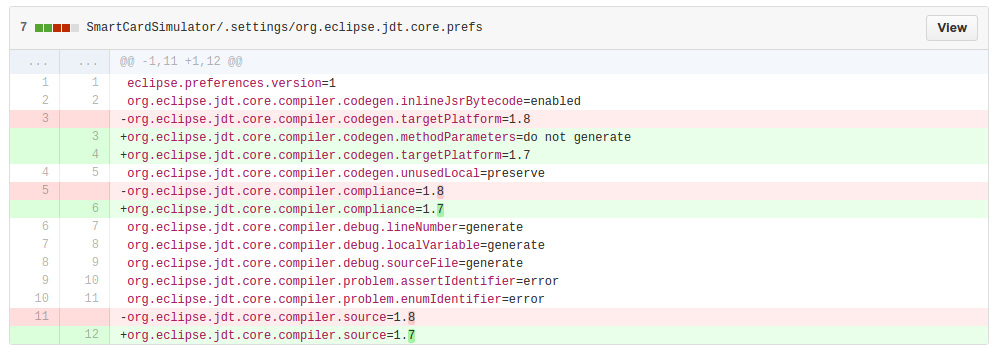
\includegraphics[width=.8\linewidth]{figures/fix_java_version.png}
	\caption{Project properties change to fix SCS Java version issue}
	\label{fig:fix_java_version}
\end{figure}

\clearpage

\section{SCS Pin shown in Command Line} - While using the Smart Card Simluator in Linux environments, the SCS Pin was being printed to the command line, after clicking the \textit{Generate Tan} button. This is a security flaw and can compromise privacy. This has been fixed and all the stack traces have been modified to simple print statements. Refer figure \ref{fig:fix_scs_pin_shown} for the code change. \\ \\ \\

\begin{figure}[ht]
	\centering
	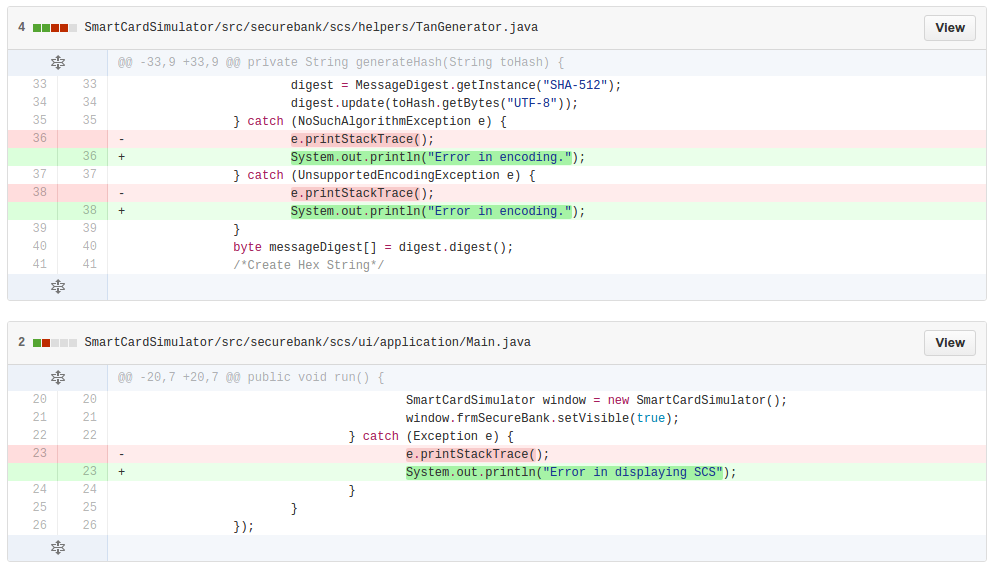
\includegraphics[width=.8\linewidth]{figures/fix_scs_pin_shown.png}
	\caption{Code change to fix SCS Pin shown}
	\label{fig:fix_scs_pin_shown}
\end{figure}

\clearpage 

\section{Business Logic Data Validation} - We do not consider this as an issue, as the current implementation is similar to the real-world working. In real working, the account name does not matter and does not  have to match the account number used at the time of transaction. The only relevant factor is the \textit{Account Number} of the recipient.
If the transfers were performed through the addition of beneficiaries, then the concept of \textit{Recipient Name} would make more sense. However, since we do not have this implementation, this could be termed as an improvement for the future.

\section{Weak SSL/TLS Ciphers} - This was resolved by prohibiting the use of old SSL versions. For that the line \code{SSLProtocol all -SSLv2 -SSLv3} was added to the virtual host configuration.

\section{Error Codes} - This would have been resolved by using custom error pages. We tried to fix this by adding \code{ErrorDocument <code> <custom error page>} to our \code{.htaccess} file, but it did not show the expected result. Therefore up to this point it is not fixed.

\section{Guessable User Account} - This was a minor issue, where-in different error messages were displayed to the user upon failed login. The error message is now made consistent to show \enquote{Either the e-mail or the password is wrong}. So it is not possible to guess whether the account does not exist or the password is wrong.

The code change for this fix happened to just be modification of the message, as can be seen in the figure \ref{fig:fix_guessable_account}.

\begin{figure}[ht]
	\centering
	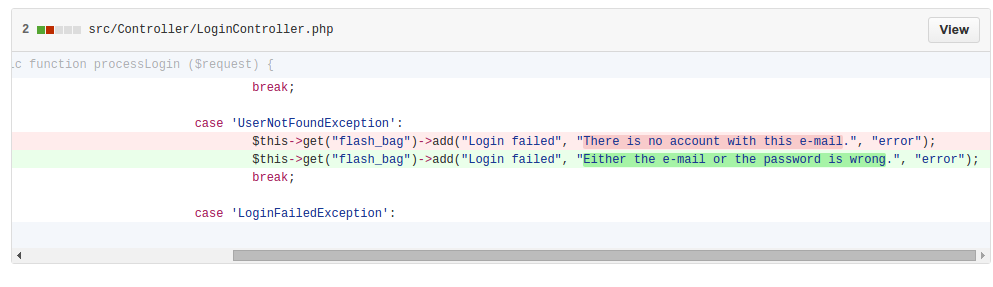
\includegraphics[width=.8\linewidth]{figures/fix_guessable_account.png}
	\caption{Code change to fix Guessable User Account}
	\label{fig:fix_guessable_account}
\end{figure}

\clearpage